
%(BEGIN_QUESTION)
% Copyright 2010, Tony R. Kuphaldt, released under the Creative Commons Attribution License (v 1.0)
% This means you may do almost anything with this work of mine, so long as you give me proper credit

Calculate what the voltmeter will register when connected to the terminals in the RTD head, if the transmitter in this 3-wire RTD circuit uses a 0.2 mA current source to ``excite'' the RTD circuit:

$$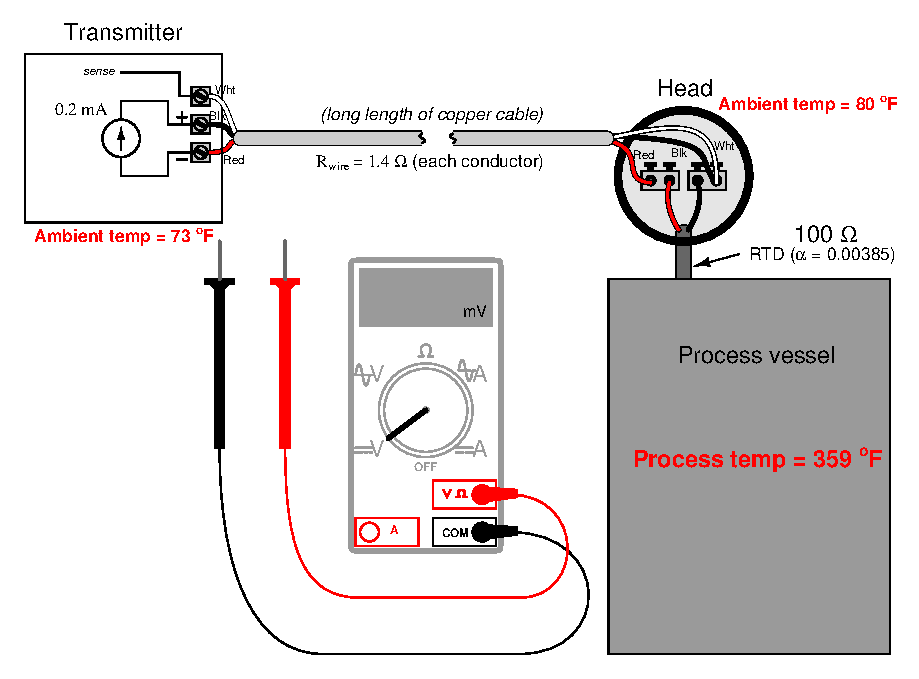
\includegraphics[width=15.5cm]{i00637x01.eps}$$

$V_{meter}$ = \underbar{\hskip 50pt} millivolts

\underbar{file i00637}
%(END_QUESTION)





%(BEGIN_ANSWER)

$V_{meter}$ = {\bf 33.818} millivolts (based on table)

\vskip 10pt

$V_{meter}$ = {\bf 33.988} millivolts (based on formula)

%(END_ANSWER)





%(BEGIN_NOTES)

{\bf This question is intended for exams only and not worksheets!}.

%(END_NOTES)

